
\chapter{光的波动性}\label{chp:light_wave_properties}
从古代起,人们就已经熟悉光现象了。
但是,光究竟是什么呢?这却是一个不容易回答的问题。
人类对光的本性的认识,经历了漫长而曲折的道路,有一个辩证发展的过程。
根据事实建立学说,发展学说,或者决定学说的取舍;发现新的事实,再建立新的学说。
人们就是这样通过光的行为,经过分析研究,逐渐认识光的本性的。

在这一章和\cref{chp:particle_light}里,我们就基本上按照这种认识发展过程来介绍关于光的本性的知识。

\section{光的微粒说和波动说}
光的本性问题很早就引起了人们的注意。
到了十七世纪,形成了两种学说。
一种是牛顿主张的\Concept{微粒说},认为光是从光源发出的一种物质微粒,在均匀媒质中以一定的速度传播。
另一种是惠更斯(1629--1695)提出的\Concept{波动说},认为光是某种振动,以波的形式向周围传播。

微粒说很容易解释光的直进现象,解释光的反射也很容易,因为小球跟光滑平面发生弹性碰撞时的反射规律跟光的反射定律相同。
然而微粒说在解释一束光射到两种媒质分界面处会同时发生反射和折射的现象时,却发生了很大的困难。
因为根据微粒说,光在镜面上发生反射,是由于光粒子受到镜面的推斥;发生折射,是由于受到折射物质表面的吸引。
在同时发生反射和折射的情况下,又怎样用推斥和吸引来解释呢?波动说却比较容易解释这种现象,因为人们知道这是波经常发生的现象。
用水槽和一些简单仪器做实验就可以看到水波同时发生反射和折射的现象,并且可以查明水波的反射和折射规律跟光非常相似。
然而波动说在解释光的直进现象时却遇到了困难,因为人们知道波能够绕障碍物,不会象光那样在物体的后面留下清晰的影子。

光的微粒说和波动说当时各有成功的一面,但都不能完满地解释当时知道的各种光现象。
只是由于牛顿在学术界有很高的声望,致使微粒说在一百多年的长时期里一直占着主导地位,波动说发展得很慢。
到了十九世纪初,人们成功地在实验中观察到了光的干涉、衍射现象,这是波的特征,无法用微粒说来解释,于是波动说得到了公认,光的波动理论也就迅速发展起来。

下面我们就来研究表明光的波动性的各种现象。

\section{光的干涉}
我们在力学中学过了波的干涉,研究过水波和声波的干涉现象。
我们知道,干涉是波特有的现象,只有频率相同、相差恒定的波源——相干波源才能产生稳定的干涉现象。
对于水波或声波,相干波源是容易得到的。
但是,要找到符合相干条件的两个相干光源却很困难。
在室内点两支蜡烛或两盏电灯,只看到墙壁被均匀照亮,丝毫看不到光的干涉现象。
当然,我们不应该因此就得出光不具有波动性的结论。
因为这些光源都是独立发光的,甚至同一光源的两个发光部分,我们也无法使它们具有相同的频率和恒定的相差,所以,即使光具有波动性,这样的两个光源也不会产生稳定的干涉现象,无法看到干涉图样。

\subsection{光的干涉}

1801 年英国物理学家托马斯·杨(1773--1829)首先巧妙而简单地解决了相干光源的问题,成功地观察到了光的干涉现象。
\begin{figure}
  \includegraphics{6-1.pdf}
  \caption{杨氏实验}\label{fig:6-1}
\end{figure}

杨氏的办法是把点光源发出的一束光分成两束,以保证它们具有相同的频率和恒定的相差。
实验做法如下。
让太阳光照射到一个有小孔的屏上(\cref{fig:6-1}),这个小孔就成了一个
“点光源”。
光从小孔出来后,照射到第二个屏的两个小孔上,这两个小孔离得很近,而且与前一小孔的距离相等。
因此,如果光足某种波动,那么任何时刻从前一小孔发出的光波都会同时传到这两个小孔,所以这两个小孔处的光振动不但频率相同,而且总是同相的。
这两个小孔就成了两个相干光源,它们发出的光在像屏某处叠加时,如果同相,光就加强,如果反相,光就减弱或抵消,因此应该产生明暗条纹。
实验果然产生了预期的结果,在像屏上看到了彩色的干涉条纹。

后来用狭缝代替小孔,用单色光代替太阳光来做实验,得到更清晰的明暗条纹,这就是著名的杨氏双缝干涉实验。
\cref{fig:6-2} 是双缝干涉的装置和产生干涉图样的示意图。
\begin{figure}
  \includegraphics{6-2.pdf}
  \caption{双缝干涉}\label{fig:6-2}
\end{figure}

\begin{figure}
  \includegraphics{6-3.pdf}
  \caption{}\label{fig:6-3}
\end{figure}
微粒说不能解释光的干涉现象,波动说则可以作出完善的解释,并能够根据双缝的距离和缝到屏的距离以及波长计算出屏上出现明暗条纹的位置。
\cref{fig:6-3} 是用波动说研究双缝干涉的图。
设两个缝 $S_1$ 和 $S_2$ 的距离为 $d$,到屏的距离为 $l$,且 $l\gg d$。
$O$ 是 $S_1S_2$ 的中垂线与屏的交点,$O$ 到 $S_1$、$S_2$ 的距离相等。
从 $S_1$、$S_2$ 射出的光波到达 $O$ 点经过的路程相等,所以两列波到达 $O$ 点时相差为零,也就是说,是同相的,它们互相加强,在 $O$ 点出现亮条纹,叫做中央亮纹。
现在我们来研究离 $O$ 点距离为 $x$ 的 $P$ 点的情况。
$P$ 到 $S_1$、$S_2$ 的距离分别为 $r_1$、$r_2$。
从 $S_1$、$S_2$ 发出的光波到达 $P$ 点的路程差是
\[\delta =r_2-r_1. \]
从图中可以看出,
\[r^2_1=l^2+\left(x-\frac{d}{2}\right)^2,\qquad r^2_2=l^2+\left(x+\frac{d}{2}\right)^2.\]
两式相减,可得
\[r^2_2-r^2_1=(r_2-r_1)(r_2+r_1)=2dx.\]
由于 $l\gg d$,且 $l\gg x$,因此 $r_2+r_1\approx 2l$,所以
\[\delta=\frac{d}{l}x.\]
如果路程差 $\delta$ 等于波长 $\lambda$ 的整数倍,两列波到达 $P$ 点时同相,因而互相加强,这里就出现亮条纹;如果路程差 $\delta$ 等于半波长 $\lambda/2$ 的奇数倍,两列波到达 $P$ 点时反相,因而互相削弱,这里就出现暗条纹。

所以,在屏上满足
\[x=\pm k\frac{l}{d}\lambda, \qquad k=0,1,2,\ldots \]
的地方出现亮条纹。
当 $k=0$ 时,$x=0$ 为中央亮纹;当 $k=1,2,\ldots$ 时,分别为中央亮纹两边的第 1 条、第 2 条……亮条纹。

在满足
\[x=\pm(2k-1)\frac{l}{d}\cdot \frac{\lambda}{2},\qquad k=1,2,\ldots \]
的地方出现暗条纹,当 $k=1,2,\ldots$ 时,分别为中央亮纹两边的第 1 条、第 2 条……暗条纹。

相邻两条亮纹(或暗纹)间的距离 $\Delta x$ 为
\[\Delta x=\frac{l}{d}\lambda.\]
可见,相邻两条亮纹(或暗纹)间的距离是相等的,从上式看出,在 $d$ 和 $\lambda$ 相同的情况下,干涉条纹间的距离 $\Delta x$ 跟波长 $\lambda$ 有关系。
用不同的色光做实验,可以看到 $\Delta x$ 的宽度不同,红光的最宽,紫光的最窄。
这表明不同色光的波长不同,红光的波长最长,紫光的波长最短。
用白光作光源时,由于各色光的波长不同,$\Delta x$ 的宽度也不同,因此在中央白色亮纹两边出现彩色条纹。

上面的公式提供了一种测量光波波长的方法:测出 $n$ 条亮纹(或暗纹)间的距离 $a$,算出相邻两条亮纹(或暗纹)间的距离
\[\Delta x=\frac{a}{n-1},\]
再测出 $d$ 和 $l$ 的值,就可以算出波长 $\lambda$。

\subsection{波长和频率}

我们知道,波长与频率的乘积等于波速。
各种色光在真空中的速度都等于 $c$,如果用 $\nu$ 表示光波的频率;则有 $c=\lambda\nu$。
由于各种色光的波长不同,可见它们的频率也不相同。
红光的波长最长,频率最小;紫光的波长最短,频率最大。
\cref{tab:6-1} 是各种色光的频率和在真空中波长的范围:
\begin{table}
  \caption{各种色光的频率和在真空中波长的范围}\label{tab:6-1}
\begin{tblr}{colspec={cX[c]X[c]cX[c]X[c]},hline{2}=0.8pt,vline{4}=1.2pt}
色光 & 波长 (\unit{\micro m})& 频率(\qty{e14}{Hz})& 色光  & 波长 (\unit{\micro m})& 频率(\qty{e14}{Hz})\\
红   & \numrange{0.77}{0.62}   & \numrange{3.9}{4.8}  & 绿    & \numrange{0.58}{0.49}   & \numrange{5.2}{6.1}  \\
橙   & \numrange{0.62}{0.60}   & \numrange{4.8}{5.0}  & 蓝—靛 & \numrange{0.49}{0.45}   & \numrange{6.1}{6.7}  \\
黄   & \numrange{0.60}{0.58}   & \numrange{5.0}{5.2}  & 紫    & \numrange{0.45}{0.39}   & \numrange{6.7}{7.7}  \\
\end{tblr}
\end{table}

光的波长也常用埃(\AA)作单位,$\qty{1}{\text{\AA}}=\qty{e-10}{m}$。
但埃不是国际制单位。

\section{薄膜干涉及其应用}
\subsection{薄膜干涉}
把金属丝圆环在肥皂液里蘸一下,环上就形成一层肥皂液薄膜。
用单色光照射薄膜,薄膜上就产生明暗相间的干涉条纹(\cref{fig:6-4})。
产生这种现象是由于照射到膜上的光会从膜的前表面和后表面分别反射回来,形成两列波,这两列波是由同一入射波产生的,因此频率相同,相差恒定,能够产生干涉。
竖立的肥皂薄膜在重力作用下成为上薄下厚的楔形,在薄膜的某些地方,反射回来的两列波恰好波峰和波峰(或者波谷和波谷)叠加,光振动加强,产生亮条纹;在另外一些地方,恰好波峰和波谷叠加,光振动削弱,产生暗条纹,这就是薄膜干涉的原因。
\begin{figure}
  \includegraphics{6-4.pdf}
  \caption{肥皂液膜上光的干涉}\label{fig:6-4}
\end{figure}

肥皂泡在太阳光照耀下会出现彩色的条纹,也是由薄膜干涉产生的。
白光中每种色光的波长不同,所以在薄膜某一厚度的地方,某一波长的反射光互相加强,就出现这种色光的亮纹;在另一厚度的地方,另一波长的反射光互相加强,就出现另一色光的亮纹。
这样,在薄膜上就出现了不同颜色的条纹。

\subsection{检查精密零件的表面质量}
\begin{figure}
  \begin{minipage}[b]{0.45\linewidth}\centering
    \includegraphics{6-5a.pdf}
    \subcaption{}\label{fig:6-5a}
  \end{minipage}
  \begin{minipage}[b]{0.45\linewidth}\centering
    \includegraphics{6-5b.pdf}
    \subcaption{}\label{fig:6-5b}
  \end{minipage}
  \caption{用干涉法检查表面}\label{fig:6-5}
\end{figure}

各种精密零件,例如光学元件,对表面加工的质量要求很高,一般精度要求在几分之一光
波波长之内。
这样的表面需要用干涉法来检验。
如果被检查的表面是一个平面,可以在它的上面放一个透明的标准样板,并在一端垫一薄片,使样板的标准平面和被检查的平面间形成一个劈形的空气薄层(\cref{fig:6-5a})。
用单色光从上面照射,入射光从空气层的上下表面反射出两列光波,于是从反射光中就会看到干涉条纹。
如果被测表面是平的,产生的干涉条纹就是一组平行的直线;如果被测表面某些地方不平,产生的干涉条纹就要发生弯曲(\cref{fig:6-5b})。
从干涉条纹弯曲的方向和程度还可以了解被测表面的不平情况。
这种测量的精度可达 \qty{e-6}{cm}。

\subsection{增透膜}

现代光学装置,如摄影机、电影放映机、潜水艇的潜望镜等,都是由许多透镜和棱镜组成的。
光进入这些装置时,在每个镜面上都有一部分光被反射,使得通过装置的光减少,结果成的像就不清晰。
计算表明,如果一个装置中包含有六个透镜,那么将有 50\% 左右的光被反射,为了减少光在元件表面上的反射损失,提高成像的质量,可在元件表面涂上一层透明薄膜(一般用氟化镁)。
当薄膜厚度是入射光在薄膜介质中波长的 $1/4$ 时,在薄膜的两个面上反射的光,路程差恰好等于半个波长,因而互相抵消,这就大大减少了光的反射损失,增强了透射光的强度。这种薄膜叫做增透膜。

在通常情况下入射光为白光,增透膜的厚度只能使一定波长的光反射时互相抵消,不可能使白光中的所有波长的光都互相抵消。
在选择增透膜的厚度时,一般是使光谱中部的绿光在直入射时互相抵消,因为人的视觉对这种光最敏感。
这时光谱边缘部分的红光和紫光并没有完全抵消,所以涂有增透膜的光学镜头呈淡紫色。

\begin{Reading}{全息照相}
同学们从报刊杂志上可能看到过全息照相这个名词,知道全息照相是一种新的照相技术。
那么,什么是全息照相?
它与普通照相有什么不同?
下面我们就来介绍一下这个问题。

我们知道,普通照相是把照相机的镜头对着被拍摄的物体,让从物体上反射的光进入镜头,在感光底片上产生物体的像。
感光底片上记录的是从物体上各点反射出来的光的强度。

但是,光是一种波,从被摄物体上各点反射出来的光不仅强度(它正比于光波振幅的平方)不同,而且位相也不同。
全息照相就是一种既记录反射光的强度,又记录反射光的位相的照相术,。
这种照相术记录的是光波的振幅和位相的全部信息,所以称为全息照相。
\begin{figurehere}
  \includegraphics{6-6.pdf}
  \caption{全息照相原理示意图}\label{fig:6-6}
\end{figurehere}

全息照相是应用光的干涉来实现的。
它用激光(是良好的相干光)作光源。
全息照相的原理如\cref{fig:6-6} 所示,激光束被分成两部分:一部分射向被摄物体,另一部分射向反射镜(这束光叫做参考光束)。
从物体上反射出来的光(叫做物光束)具有不同的振幅和位相,物光束和从反射镜来的参考光束都射到感光片上,两束光发生干涉,在感光片上产生明暗的干涉条纹,感光片就成了全息照片。
干涉条纹的明暗记录了干涉后光的强度,干涉条纹的形状记录了两束光的位相关系。

从全息照片的干涉条纹上不能直接看到物体的像,为了现出物体的像,必须用激光束(参考光束)去照射全息照片,当参考光束通过全息照片时,便复现出物光束的全部信息,于是就能看到物体的像。

全息照相较之普通照相有许多优点。
第一,它再现出来的像是跟原来物体一模一样的逼真的立体像,跟观察实物完全一样;第二,把全息照片分成若干小块,每一小块都可以完整地现出原来物体的像,所以全息照片即使有缺损,也不会使像失真;第三,在同一张感光片上可以重迭记录许多像,这些像能够互不干扰地单独显示出来。

全息照相技术有重要的实际应用。
全息照相在一张感光片上可以重叠记录许多像,这为信息的大容量高密度储存提供了可能,例如用全息照相方法可以把一本几百页的书的内容存储在只有指甲大小的全息照片上。
全息照相在精密测量、无损检验、显微术等方面也得到应用。
随着全息照相技术的发展,它将会得到更广泛的应用。
\end{Reading}

\begin{Practice}
\begin{question}
  \item 绿光的干涉条纹与红光的干涉条纹有什么不同?用白光做干涉实验,为什么会得到彩色的干涉条纹?在彩色条纹中最靠近中央亮纹的是哪种颜色的条纹?为什么?
  \item 在杨氏双缝实验中,保持双缝到屏的距离不变,调节双缝间的距离,当距离增大时,干涉条纹间的距离将变\underline{\qquad};当距离减小时,干涉条纹间的距离将变\underline{\qquad}。
  \item 色光从真空进入媒质后,频率不变,但传播速度减小了,波长将如何变化?
  \item 用单色光做双缝干涉实验,测得双缝间的距离为 \qty{0.4}{mm},双缝到屏的距离为 \qty{1}{m},干涉条纹的间距为 \qty{1.5}{mm},求所用光波的波长。
  \item 取两块平玻璃板,用手指把它们紧紧捏在一起,会从玻璃板面上看到许多彩色花纹;改变手指用力的大小,花纹的颜色和形状也随着改变,做这个实验,并解释看到的现象。
\end{question}
\end{Practice}

\section{光的衍射}
\subsection{光的衍射}
我们知道,波能够绕过障碍物产生衍射,衍射也是波特有的现象。
并且知道只有障碍物或孔的尺寸跟波长相差不多时,才能明显地观察到波的衍射现象。

光既然是一种波动,那么,光在传播中是否也能产生衍射现象呢?从前面讲的光的干涉实验知道,光波的波长是很短的,只有十分之几微米,通常的物体都比它大得多,因此很难看到光的衍射现象。
但是,当光射向一个针孔、一条狭缝、一根细丝时,就会出现衍射现象。

取一个不透光的屏,在屏中间开一个较大的圆孔。
用点光源照射,在像屏上就出现一个明亮的圆形光斑(\cref{fig:6-7a})。
显然,这是光沿直线传播的结果。
圆孔小一些,可以看到像屏上的光斑也随着减小(\cref{fig:6-7b})。
但是,圆孔很小(直径小于 \qty{0.1}{mm})时,像屏上的光斑不仅不减小,反而变大了,而且光斑的亮度也变得不均匀,成为一些明暗相间的圆环(\cref{fig:6-7c})。
这些圆环的面积,远远超过了光按直线传播所能照到的范围,就是说光绕到小孔以外的区域中去了。
这就是光通过小孔产生的衍射现象。
\begin{figure}
  \begin{minipage}{0.1\linewidth}
    \subcaption{}\label{fig:6-7a}
  \end{minipage}%
  \begin{minipage}{0.65\linewidth}\centering
    \includegraphics{6-7a.pdf}
  \end{minipage}\par
  \begin{minipage}{0.1\linewidth}
    \subcaption{}\label{fig:6-7b}
  \end{minipage}%
  \begin{minipage}{0.65\linewidth}\centering
    \includegraphics{6-7b.pdf}
  \end{minipage}\par
  \begin{minipage}{0.1\linewidth}
    \subcaption{}\label{fig:6-7c}
  \end{minipage}%
  \begin{minipage}{0.65\linewidth}\centering
    \includegraphics{6-7c.pdf}
  \end{minipage}\par
  \caption{光通过小圆孔的衍射}\label{fig:6-7}
\end{figure}

如果在不透明的屏上装一个宽度可以调节的狭缝,代替上面实验中的小圆孔,重做实验,可以看到:当缝比较宽时,光沿直线传播,在像屏上出现一条亮线;当缝很窄时,光通过缝
后就明显地偏离了直线传播的方向,像屏上被照亮的范围变宽,并且出现了明暗相间的条纹。
这是光通过狭缝时产生的衍射现象。

光的衍射现象进一步证明了光具有波动性,对建立光的波动说起了重要的作用。
关于这个问题,历史上曾有过一段趣事。
十九世纪初,法国物理学家菲涅耳(1788--1827)利用波动理论对光的衍射现象作出了数学分析。
当时一位反对波动说的数学家泊松从菲涅耳的分析得出结论:如果菲涅耳的理论是正确的,那么把一个小的圆盘状物体放在光束中,在距这个圆盘一定距离的像屏上,圆盘的影的中心应当出现一个亮斑:人们从未看到过和听说过这种现象,因而认为这是荒谬的。
于是微粒说的拥护者们认为可以驳倒波动说了。
菲涅耳接受了这一挑战,精心研究,奇迹终于出现了,实验证明盘影的中心确实有亮斑(\cref{fig:6-8})。
微粒说无法解释这种奇特的现象,而波动说却能作出完满的解释。
菲涅耳的理论和实验使波动说获得了巨大的成功。

\begin{figure}
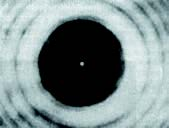
\includegraphics[width=0.6\linewidth]{6-8.jpg}
\caption{不透明盘产生的衍射,影子的中心有一个亮斑(泊松亮斑)}\label{fig:6-8}
\end{figure}

\subsection{衍射光栅}
\begin{figure}
  \begin{minipage}{0.24\linewidth}\centering
    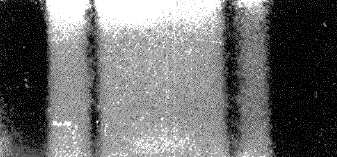
\includegraphics[width=\linewidth]{6-9a.png}
    \subcaption{1 缝}\label{fig:6-9a}
  \end{minipage} 
  \begin{minipage}{0.24\linewidth}\centering
    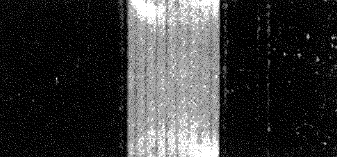
\includegraphics[width=\linewidth]{6-9b.png}
    \subcaption{2 缝}\label{fig:6-9b}
  \end{minipage} 
  \begin{minipage}{0.24\linewidth}\centering
    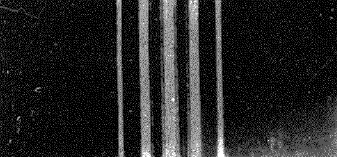
\includegraphics[width=\linewidth]{6-9c.png}
    \subcaption{5 缝}\label{fig:6-9c}
  \end{minipage} 
  \begin{minipage}{0.24\linewidth}\centering
    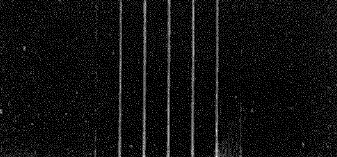
\includegraphics[width=\linewidth]{6-9d.png}
    \subcaption{20 缝}\label{fig:6-9d}
  \end{minipage}
	\caption{衍射条纹随着缝数增加而变窄}\label{fig:6-9}
\end{figure}

光通过单狭缝产生的衍射条纹的位置跟光波的波长有关,因此,利用衍射条纹也可以测定波长。但是单缝的衍射条纹比较宽,测量的结果很不精确。
为了精确测出光波的波长,可以增加缝数。
因为缝数增加以后,从各条单缝衍射出来的光波要互相干涉,结果使明条纹变窄了。
这个问题的具体分析比较复杂,我们在这里就不讲了。
从\cref{fig:6-9} 中可以清楚地看到明条纹随着缝数增加而变窄的情形。

光学仪器中用的衍射光栅就是根据这个原理制成的。
常用的透射光栅是在玻璃片上刻有许多等宽而又等间距的平行刻痕,其中刻痕是不透光的部分(\cref{fig:6-10})。
实用的衍射光栅一般在每毫米内有几十条乃至上千条狭缝。
光栅产生的衍射条纹又窄又亮,可以精确地测定光波的波长。
不同波长的光通过光栅后产生的衍射条纹的位置不同,因此,利用光栅可以把不同波长的色光分开,就是说,光栅跟棱镜一样具有分光作用,用它可以产生光谱,这也是光栅的一个用途。
\begin{figure}
  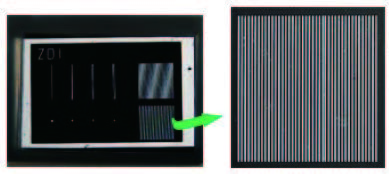
\includegraphics[width=0.97\linewidth]{6-10.jpg}
  \caption{衍射光栅}\label{fig:6-10}
\end{figure}

\begin{Practice}
\begin{question}
  \item 为什么隔着墙能听到墙那边人的说话声,但看不见人?
  \item 光的衍射现象跟光的直线传播是否矛盾?在什么情况下光沿直线传播?
  \item 把两支铅笔并在一起,中间留一条狭缝,放在眼前,进过这条狭缝去看远处的日光灯,使狭缝的方向跟灯管平行,就看到许多条平行的彩色条纹,做这个实验,并解释看到的现象。
\end{question}
\end{Practice}

\section{光的偏振}
光的干涉和衍射现象清楚地表明光是一种波,我们知道,波有纵波和横波,这两种波都能够产生干涉和衍射现象,那么,光波究竟是纵波还是横波呢?

我们先用机械波来说明纵波和横波的主要区别,沿着绳传播的横波,如果在它传播的方向上放上带有狭缝的木板(\cref{fig:6-11}),只要狭缝的方向跟绳的振动方向相同,绳上的横波就可以毫无阻碍地传过去;如果把狭缝的方向旋转 \ang{90},绳上的横波就不能通过了,这种现象叫做横波的\Concept{偏振}。
纵波是沿着波的传播方向振动的,不论狭缝方向如何,纵波都可以传过去,不会发生偏振现象(\cref{fig:6-12})。
\begin{figure}
  \begin{minipage}[b]{0.48\linewidth}\centering
    \includegraphics{6-11a.pdf}
    \subcaption{}\label{fig:6-11a}
  \end{minipage}
  \begin{minipage}[b]{0.48\linewidth}\centering
    \includegraphics{6-11b.pdf}
    \subcaption{}\label{fig:6-11b}
  \end{minipage}
  \caption{横波的偏振}\label{fig:6-11}
\end{figure}
\begin{figure}
  \includegraphics{6-12.pdf}
  \caption{纵波没有偏振现象}\label{fig:6-12}
\end{figure}

光是否产生偏振现象呢?十九世纪法国科学家马吕(1775--1812)发现,光也能够产生偏振现象。
我们可以用下面的方法来观察这一现象。

取一块电气石晶体薄片或人造偏振片\footnote{常用的一种人造偏振片是把聚乙烯醇薄膜在碘溶液里浸泡后,在较高的温度下拉伸,再烘干制成的。},通过它观察太阳光或灯光,可以看到它是透明的。以入射光线为轴旋转晶片,这时着到的透射光的强度并不发生变化。
再取一个同样的晶片,把它放在前一晶片的后面,通过它去观察从前一晶片透射过来的光,就会发现,从第二个晶片透射过来的光的强度跟两晶片的相对方向有关。
把前一晶片固定,以入射光线为轴旋转后一晶片时,从后一晶片透射过来的光的强度发生周期性的变化:后一晶片转到某一方向时,透射光最强(\cref{fig:6-13a});再旋转 \ang{90},转到跟前一方向垂直时,透射光最弱,几乎等于零(\cref{fig:6-13b})。
\begin{figure}
  \begin{minipage}{0.1\linewidth}\raggedleft
    \subcaption{}\label{fig:6-13a}
  \end{minipage}%
  \begin{minipage}{0.6\linewidth}\centering
    \includegraphics{6-13a.pdf}
  \end{minipage}\par\medskip
  \begin{minipage}{0.1\linewidth}\raggedleft
    \subcaption{}\label{fig:6-13b}
  \end{minipage}%
  \begin{minipage}{0.6\linewidth}\centering
    \includegraphics{6-13b.pdf}
  \end{minipage}
  \caption{光的偏振}\label{fig:6-13}
\end{figure}

把上述光现象跟机械波的偏振现象相比较,表明光通过晶片时产生偏振现象。
只有横波才产生偏振现象,所以光波是横波。

上面实验中的现象可以解释如下。
太阳、电灯等普通光源发出的光,包含着在垂直于传播方向上沿一切方向振动的光,并没有一个占优势的方向,也就是说,沿着各个方向振动的光波强度都相同,这种光叫做\Concept{自然光}。
自然光通过第一个晶片(叫做起偏器)后,相当于被一个“狭缝”卡了一下,只有振动方向跟“狭缝”方向一致的光波才能通过(\cref{fig:6-13}),这种振动方向一定的光叫做\Concept{偏振光}。
每个偏振片上都有一条标线,表示的就是偏振片允许通过的偏振光的振动方向,这个方向叫做偏振片的偏振化方向。
自然光通过第一个晶片后虽然变成了偏振光,但由于自然光中沿各个方向振动的光波强度都相同,所以不论晶片转到什么方向,都会有相同强度的光透射过来。
再通过第二个晶片(叫做检偏器)去观察,情形就不同了。
不论旋转哪个晶片,两晶片的偏振化方向一致时,透射光最强,两晶片的偏振化方向互相垂直时,透射光最弱。

光的偏振现象并不是罕见的。
我们通常看到的绝大部分光,除了从光源直接射来的,基本上都是偏振光,只是我们眼睛不能鉴别罢了。
如果通过偏振片去观察从玻璃或水面反射的光,旋转偏振片,就会发现透射光的强度也发生周期性的变化,从而知道反射光是偏振光。

光的偏振现象在技术中有很多应用。
例如,在拍摄水面下的景物或展览橱窗中的陈列品的照片时,由于从水面或窗玻璃会发出很强的反射光,使得水面下的景物和橱窗中的陈列品看不清楚,摄出的照片也模糊不清。
如果在照相机镜头上加一个偏振片,使偏振片的偏振化方向与反射光的垂直,就可以把这些反射光滤掉,而摄得清晰的照片。
汽车在夜间行车时,迎面开来的车灯的光常常使司机看不清路面,容易发生事故。
如果在每辆汽车的车灯玻璃上和司机座席前面的窗玻璃上各安上一块偏振片,并使它们的偏振化方向都跟水平方向成 \ang{45} 角(\cref{fig:6-14}),就可以解决这个问题。
这时,从对面车灯射来的偏振光,由于振动方向跟司机自己座前窗玻璃上偏振片的偏振化方向垂直,所以不会射进司机眼里。
而从自已的车灯射出去的偏振光,由于振动方向跟自己的窗玻璃上偏振片的偏振化方向相同,所以司机仍能看清自己车灯照亮的路面和物体。

\begin{figure}
  \includegraphics{6-14.pdf}
  \caption{汽车车灯和窗玻璃上的偏振片}\label{fig:6-14}
\end{figure}

\begin{Reading}{偏振光与立体电影}
看立体电影,要戴上一副特殊的眼镜,这样从银幕上看到的人物和自然景物的影像才有立体感,犹如身临其境一般。
如果取下眼镜,银幕上的图象就模糊不清了。
这是一副什么眼镜?
为什么能使我们看到的影像有立体感?
学习了偏振光的知识,就可以明白它的原理了。

为了说明立体电影的原理,首先得说说用两只眼睛看物体跟用一只眼睛看物体的区别。
用两只眼睛看物体时,由于两眼看到的同一物体略有差别,因而产生立体感。
只用一只眼睛看物体,就没有立体感。

普通电影是用一架摄影机拍摄,一架放映机放映的,银幕上的画面是一幅平面图像。
立体电影是用两架摄影机并排在一起,同时拍下同一景物的两幅图象,由于两架摄影机对景物的角度不同,所以拍下的两幅图像略有差别,就如同两眼看到的同一物体略有差别一样。
放映时,用两架放映机把两架摄影机拍下的两组影片同步放映,使略有差别的两幅图像重叠在银幕上。
这时如果用眼睛直接观看,看到的画面是模糊不清的,要看到立体电影,需要运用光的偏振知识,使两眼各看到一幅图像。
在每架放映机前装一块偏振镜(\cref{fig:6-15}),其作用相当于起偏器,从两架放映机发出的带有影像的两束光,通过偏振镜后,就成了偏振光。
左右两架放映机前的偏振镜的偏振化方向互相垂直,因此产生的两束偏振光的偏振方向也互相垂直。
这两束偏振光投射到银幕上再反射到观众,偏振方向不改变。
观众戴的眼镜是一副偏光眼镜,相当于检偏器,偏光眼镜的两只镜片的偏振化方向也是互相垂直的,而且左眼镜片的偏振化方向跟左边放映机前偏振镜的一致,右眼镜片的偏振化方向跟右边放映机前偏振镜的一致。
这样,左眼只能看到左机映出的画面,右眼只能看到右机映出的画面,两眼看到的画面略有差别,因而产生立体感。
\begin{figurehere}
  \begin{minipage}{\linewidth}\centering
  \includegraphics{6-15.pdf}
  \caption{立体电影}\label{fig:6-15}
  \end{minipage}
\end{figurehere}
\end{Reading}

\section{光的电磁说}
十九世纪初,杨氏、菲涅耳等对光的干涉和衍射的研究,使光的波动说获得了很大的成功,逐渐为人们所接受。
物理学家们继续发展和完善光的波动说,试图对光波作出进一步的说明。
当时人们只了解在媒质中传播的机械波,以为光波也是这种机械波。
但是,一切机械波,包括声波在内,都需要有传播的媒质,在真空中是不能传播的。
光却能够在真空中传播,从太阳和其他恒星发出的光,能够穿过辽阔的宇宙空间传到地球上来。
那么,光是通过什么媒质传过来的呢?为了说明光的传播问题,人们曾假设在宇宙空间里到处都充满着一种特殊的物质,叫做“以太”,认为光是通过“以太”传播的。
为了解释光波是横波、光波传播的速度很大、光波在不同媒质中的传播速度不同等问题,对“以太”这种物质的性质作了种种假设,例如,“以太”的密度应该非常小,但是又应该具有很大的弹性。
对“以太”性质所作的假设有些是互相矛盾的,很难使人相信存在这样的物质。
为了证明“以太”的存在,人们曾做过各种实验,但是都失败了,这使得认为光波是通过“以太”传播的机械波的理论陷入了困境。

1846 年,法拉第发现在磁场的作用下,偏振光的振动面会发生改变。
这个发现很重要,它表明光和电磁现象间存在着联系,启示人们把光现象和电磁现象联系起来考虑。

十九世纪六十年代,麦克斯韦在研究电磁场理论时预见了电磁波,并且指出电磁波是横波,电磁波的传播速度等于光速。
麦克斯韦根据电磁波跟光波的这些相似性指出,光波是一种电磁波,这就是\Concept{光的电磁说}。

二十多年以后,赫兹用实验证实了电磁波的存在,测得电磁波的传播速度确实等于光速,而且电磁波也能产生反射、折射、干涉、衍射、偏振等现象,其规律都跟光波的相同。
这就从实验上证实了光是一种电磁波。

前面\cref{chp:electromagnetic_wave}已经讲过,电磁波跟机械波不同,电磁波可以在真空中传播,不需要依靠别的媒质。
这就解决了光波在传播媒质上所遇到的困难。

麦克斯韦提出的光的电磁说,在物理学的发展中有很重要的意义。
它把光现象和电磁现象统一起来,指出了它们的一致性,再一次证明了自然现象之间是相互联系的。
光的电磁说使人们对光的本性的认识前进了一大步。

\section{电磁波谱}
我们已经知道,无线电波是电磁波,其波长范围从几十千米到几毫米,现在又知道了光波也是电磁波,其波长不到 \qty{1}{\micro m}。
可见,电磁波是一个很大的家族,包括的波长范围很大。
光波里能够作用于我们的眼睛并引起视觉的部分,只是一个很窄的波段,通常也叫做可见光。
正象在可闻声波范围外还存在着大量的听不见的超声波和次声波一样,在可见光波范围外还存在着大量的看不见的红外线和紫外线。

\subsection{红外线}
红外线是英国物理学家赫谢耳在 1800 年发现的,他用灵敏温度计研究光谱里各种色光的热作用时,把温度计移到光谱的红光区域外侧,它的温度上升得更高,说明那里有看不见的射线照射到温度计上,这种射线后来就叫做红外线。
给电炉丝通电,电炉丝的温度大约上升到 \qty{500}{\celsius} 以上时,才开始发出暗红色的光,随着温度的升高,它逐渐变成橙色、黄色;但在电炉丝发光之前,我们就已感到热了。
这就是它发射了红外线的缘故。
一切物体都可以发射红外线,温度较高的物体发出的红外线也较多。

红外线在工业、农业、军事、科研以及人民生活中都有广泛的应用,红外线技术已发展成为一门现代科学技术。
红外线最显著的作用是热作用,所以可以利用红外线来加热,红外线炉,红外线烤箱、红外线干燥器等,都是利用红外线来加热的。
这种加热方法的优点是能使物体从内部发热,加热效率高,效果好。
利用对红外线敏感的底片可以进行远距离摄影和高空摄影。
从卫星上用红外线对地面摄影,从照片上可以清晰地看出地面上的城市、街道、桥梁和房屋,这种摄影不受白天和夜晚的限制。
利用红外成像技术可以制成军事上用的夜视仪,使人们在漆黑的夜间能够看见目标。
一切物体,包括大地、云雾、冰块、人体、飞机和车船,都在不停地辐射红外线,并且不同的物体辐射的红外线的波长和强度不同,利用灵敏的红外线探测器吸收物体发出的红外线,然后用电子仪器对接收到的信号进行处理,就可以察知被探测物体的特征。
这种技术叫做\Concept{红外线遥感}。
利用红外线遥感技术,可以在飞机或卫星上勘测地热、寻找水源、监测森林火情、估计农作物的长势和收成、预报台风寒潮等。
红外线遥感技术的应用范围极其广泛,还在迅速发展中。

\subsection{紫外线}
紫外线是德物理学家里特在 1801 年发现的。
如果在光谱的紫外区域放一张照相底片,或者放一个光敏电阻,都能够察知紫外线的存在。
紫外线的波长比紫光还短。
一切高温物体,如太阳、弧光灯发出的光都含有紫外线,利用气体放电也可以激发紫外线。紫外线的主要作用是化学作用。
紫外线很容易使照相底片感光。
用紫外线照相能辨认出细微差别,例如可以清晰地分辨出留在纸上的指纹。
紫外线有很强的荧光效应,能使许多物质激发荧光。
日光灯和农业上诱杀害虫用的黑光灯,都是用紫外线来激发荧光物质发光的。
紫外线还有杀菌消毒作用。
医院里常用紫外线来消毒病房和手术室。
紫外线还能促进生理作用和治疗皮肤病、软骨病等。
经常在矿井下劳动的工人,适当地照射紫外线,能促进身体健康。
但过强的紫外线能伤害人的眼睛和皮肤,电焊的弧光中有强烈的紫外线,因此电焊工在工作时必须穿好工作服,并戴上防护面罩。

\subsection{伦琴射线}
比紫外线波长还短的电磁波,有伦琴射线。
德国物理学家伦琴(1845--1923)在1895年研究阴极射线的性质时,发现阴极射线的高速电子流射到玻璃管壁上,管壁会发出一种看不见的射线,这种射线的穿透本领很大,能使放在厚纸后面的荧光物质铂氰化钡发出荧光,并能使包在黑纸里的照相底片感光。
伦琴当时不知道这是什么射线,把它叫做 X 射线。
后来人们做了大量实验,发现高速电子流射到任何固体上,都会产生这种射线,并且从它产生的衍射现象知道它是波长很短的电磁波。
为了纪念伦琴,就把这种射线叫做伦琴射线。
\cref{fig:6-16} 是产生伦琴射线的装置,叫做伦琴射线管。图中的螺旋钨丝 $K$ 是它的阴极,用钨或铂制成的电极 $A$ 是它的阳极,又叫对阴极。
管里的真空程度很高,气压约为 \qtyrange{e-3}{e-5}{Pa}(\qtyrange{e-5}{e-7}{mmHg})。
用电池组或变压器给钨丝 $K$ 通电,钨丝达到赤热状态就向周围发射电子。
把管的阴阳两极接到几万伏的高压电源上,管内就产生很强的电场。
炽热钨丝发出的电子在电场力的作用下以很大的速度射到对阴极上,就从那里激发出相当强的伦琴射线。
伦琴射线穿透物质的本领跟物质的密度有关系,在工业上可以用它来检查金属部件有没有砂眼、裂纹等缺陷,在医学上可以用它来透视人体,检查体内的病变和骨折的情况。
\begin{figure}
  \includegraphics{6-16.pdf}
  \caption{伦琴射线管}\label{fig:6-16}
\end{figure}

此外,还有比伦琴射线波长更短的电磁波,那就是放射性元素放出的 $\gamma$ 射线,我们将在\cref{chp:atomic_nucleus}学习。

\subsection{电磁波谱}

无线电波、红外线、可见光、紫外线、伦琴射线、$\gamma$ 射线合起来,构成了范围非常广阔的\Concept{电磁波谱}(\cref{fig:6-17}),其中最长的波长是最短的波长的 \num{e21} 倍以上。
从图中可以看出,各种电磁波的范围已经衔接起来,并且发生了交错。
例如长波的红外线和微波已经重叠,短波的紫外线已经进入伦琴射线的区域。
总的说来,从无线电波到 $\gamma$ 射线,都是本质上相同的电磁波,它们的行为服从共同的规律。
另一方面,由于它们的频率或波长不同而又表现出不同的特性,例如,波长较长的无线电波,很容易表现出干涉、衍射等现象,但对波长越来越短的可见光、紫外线、伦琴射线、$\gamma$ 射线,要观察到它们的干涉、衍射现象,就越来越困难了。

\begin{figure}
  \includegraphics[scale=1]{6-17.pdf}
  \caption{电磁波谱}\label{fig:6-17}
\end{figure}

不同的电磁波产生的机理不同,无线电波是振荡电路中自由电子的运动产生的,红外线、可见光、紫外线是原子的外层电子受到激发后产生的,伦琴射线是原子的内层电子受到激发后产生的,$\gamma$ 射线是原子核受到激发后产生的。

\section{光谱}
光波是由原子内部运动的电子产生的。
各种物质的原子内部电子的运动情况不同,所以它们发射的光波也不同。
研究不同物质的发光和吸收光的情况,有重要的理论和实际意义,已成为一门专门的学科——光谱学。
下面简单介绍一些关于光谱的知识。

\subsection{分光镜}
\begin{figure}
  \includegraphics{6-18.pdf}
  \caption{分光镜构造原理示意图}\label{fig:6-18}
\end{figure}

观察光谱要用分光镜,这里我们先讲一下分光镜的构造原理。
\cref{fig:6-18} 是分光镜的构造原理示意图。
它是由平行光管 $A$、三棱镜 $P$ 和望远镜筒 $B$ 组成的。
平行光管 $A$ 的前方有一个宽度可以调节的狭缝 $S$,它位于透镜 $L_1$ 的焦平面\footnote{通过焦点垂直于透镜主光轴的平面,叫做透镜的焦平面。}处。
从狭缝射入的光线经透镜 $L_1$ 折射后,变成平行光线射到三棱镜 $P$ 上。
不同颜色的光经过三棱镜沿不同的折射方向射出,并在透镜 $L_2$ 后方的焦平面 $MN$ 上分别会聚成不同颜色的像(谱线)。
通过望远镜筒 $B$ 的目镜 $L_3$,就看到了放大的光谱像。
如果在 $MN$ 那里放上照相底片,就可以摄下光谱的像,具有这种装置的光谱仪器叫做摄谱仪。

\subsection{发射光谱}
物体发光直接产生的光谱叫做\Concept{发射光谱}。
发射光谱有两种类型;连续光谱和明线光谱。

连续分布的包含有从红光到紫光各种色光的光谱叫做\Concept{连续光谱}。
炽热的固体、液体和高压气体的发射光谱是连续光谱。
例如电灯丝发出的光、炽热的钢水发出的光都形成连续光谱。

只含有一些不连续的亮线的光谱叫做\Concept{明线光谱}。
明线光谱中的亮线叫做谱线,各条谱线对应于不同波长的光。
稀薄气体或金属的蒸气的发射光谱是明线光谱。
明线光谱是由游离状态的原子发射的,所以也叫\Concept{原子光谱}。

观察气体的原子光谱,可以使用光谱管(\cref{fig:6-19}),它是一支中间比较细的封闭的玻璃管,里面装有低压气体,管的两端有两个电极。
把两个电极接到高压电源上,管里稀薄气体发生辉光放电,产生一定颜色的光。
\begin{figure}
  \includegraphics{6-19.pdf}
  \caption{光谱管}\label{fig:6-19}
\end{figure}

观察固态或液态物质的原子光谱,可以把它们放到煤气灯的火焰或电弧中去烧,使它们气化后发光,就可以从分光镜中看到它们的明线光谱。

实验证明,原子不同,发射的明线光谱也不同,每种元素的原子都有一定的明线光谱。每种原子只能发出具有本身特征的某些波长的光,因此,明线光谱的谱线叫做原子的\Concept{特征谱线}。
利用原子的特征谱线可以鉴别物质和研究原子的结构。

\subsection{吸收光谱}
高温物体发出的白光(其中包含连续分布的一切波长的光)通过物质时,某些波长的光被物质吸收后产生的光谱,叫做\Concept{吸收光谱}。
例如,让弧光灯发出的白光通过温度较低的钠气(在酒精灯的灯芯上放一些食盐,食盐受热分解就会产生钠气),然后用分光镜来观察,就会看到在连续光谱的背景中有两条挨得很近的暗线。
这就是钠原子的吸收光谱。
值得注意的是,各种原子的吸收光谱中的每一条暗线都跟该种原子的发射光谱中的一条明线相对应。
这表明,低温气体原子吸收的光,恰好就是这种原子在高温时发出的光。
因此,吸收光谱中的谱线(暗线),也是原子的特征谱线,只是通常在吸收光谱中看到的特征谱线比明线光谱中的少。

\subsection{光谱分析}
由于每种原子都有自己的特征谱线,因此可以根据光谱来鉴别物质和确定它的化学组成。
这种方法叫做\Concept{光谱分析}。
做光谱分析时,可以利用发射光谱,也可以利用吸收光谱。
这种方法的优点是非常灵敏而且迅速。
某种元素在物质中的含量达 \qty{e-10}{g},就可以从光谱中发现它的特征谱线,因而能够把它检查出来。
光谱分析在科学技术中有广泛的应用。
例如,在检查半导体材料硅和锗是不是达到了高纯度的要求时,就要用到光谱分析。
在历史上,光谱分析还帮助人们发现了许多新元素。
例如,铷和铯就是从光谱中看到了以前所不知道的特征谱线而被发现的。
光谱分析对于研究天体的化学组成也很有用。
十九世纪初,在研究太阳光谱时,发现它的连续光谱中有许多暗线。
最初不知道这些暗线是怎样形成的,后来人们了解了吸收光谱的成因,才知道这是太阳内部发出的强光经过温度比较低的太阳大气层时产生的吸收光谱。
仔细分析这些暗线,把它跟各种原子的特征谱线对照,人们就知道了太阳大气层中含有氢、氦、氮、碳、氧、铁、镁、硅、钙、钠等几十种元素。

\begin{Review}
\begin{question}
  \item 十七世纪的光的波动说和微粒说各有什么成功之处和不足之处?
  \item 什么是光的干涉?什么是相干光源?
  \item 薄膜干涉现象是怎样产生的?举例说明薄膜干涉现象的应用。
  \item 什么是光的行射?日常生活中为什么不容易观察到光的衍射现象?
  \item 什么是光的偏振?光的偏振表明了什么?
  \item 确立光的电磁说,根据是什么?
  \item 无线电波、红外线、可见光、紫外线和伦琴射线,它们的波长(或频率)有什么不同?
  \item 发射光谱是怎样产生的?吸收光谱是怎样产生的?什么叫特征谱线?光谱分析的原理是什么?
\end{question}
\end{Review}

\begin{Exercise}
\begin{question}
  \item 你用哪些现象或实验来说明:
  \begin{tasks}(2)
    \task 光是一种波;
    \task 光波的波长非常短;
    \task 绿光的波长比红光的短。
  \end{tasks}
  \item 水对真空中波长为 \qty{0.656}{\micro m} 的红光的折射率为 $n_1=1.33$,而对真空中波长为 \qty{0.405}{\micro m} 的紫光的折射率为 $n_2=1.343$。求这两种波在水中的传播速度和波长。
  \item 波长为 \qty{5890}{\text{\AA}} 的黄光照在一双缝上,在距双缝为 \qty{1}{m} 的观察屏上,测得 20 个亮条纹的间距共宽 \qty{2.4}{cm},求双缝间的距离。
  \item 用波长为 \qty{0.75}{\micro m} 的红光做双缝干涉实验,双缝间的距离是 \qty{0.05}{mm},缝到屏的距离是 \qty{1}{m},相邻两条暗纹间的距离是多大?
\end{question}
\end{Exercise}